% Условная компиляция для самостоятельной работы
\ifdefined\mainfile
    % Если это часть основного файла, не добавляем начало и конец документа
\else
    \documentclass[12pt, a4paper]{report}
    \usepackage{/Users/vladbelousov/Desktop/Semestr_4-FP-NSU/Настройка/library}
    \usepackage[utf8]{inputenc} % Подключение поддержки UTF-8
    \begin{document}
\fi

%%-------------------------------%%

\textbf{Толстая линза (продолжение)} 

\[ \begin{pmatrix}
x_1 \\
V_1 
\end{pmatrix} = M^{-1 }
\begin{pmatrix}
    x_2 \\
    0 
\end{pmatrix} =
\begin{pmatrix}
m_{22} & -m_{12}\\
-m_{21} & m_{11}
\end{pmatrix}\begin{pmatrix}
    x_2\\
    0 
\end{pmatrix} 
\begin{aligned}
    \Rightarrow 
    \begin{cases}
        x_1= m_{22} x_2 \\
        V_1 = x_1 ' = - m_{21} x_2 
    \end{cases} 
    \Rightarrow
    z_1  =- \frac{x_1}{x_1' }= \frac{m_{22}}{m_{21}}  
\end{aligned}
\] 

\[ F_{\text{п} } = \frac{x_2}{x_1 '} = -\frac{x_2 }{m_{21}x_2 } = - \frac{1}{m_{21} } = F_{\text{Л} }    \] 

\[ h_1 = z_1 + F_{\text{п} } = \frac{m_{22}}{m_{21}} - \frac{1}{m_{21} } = \frac{m_{22} - 1 }{m_{21}}     \] 

, где \( h_1      \) - координата относительно \( O_1 \) первой главной плоскости.

Вывод: переднее и заднее фокусное расстояние одинаковы и равны  фокусному расстоянию толстой линзы \( = \displaystyle  - \frac{1}{m_{21}}  \) 

\begin{center}
    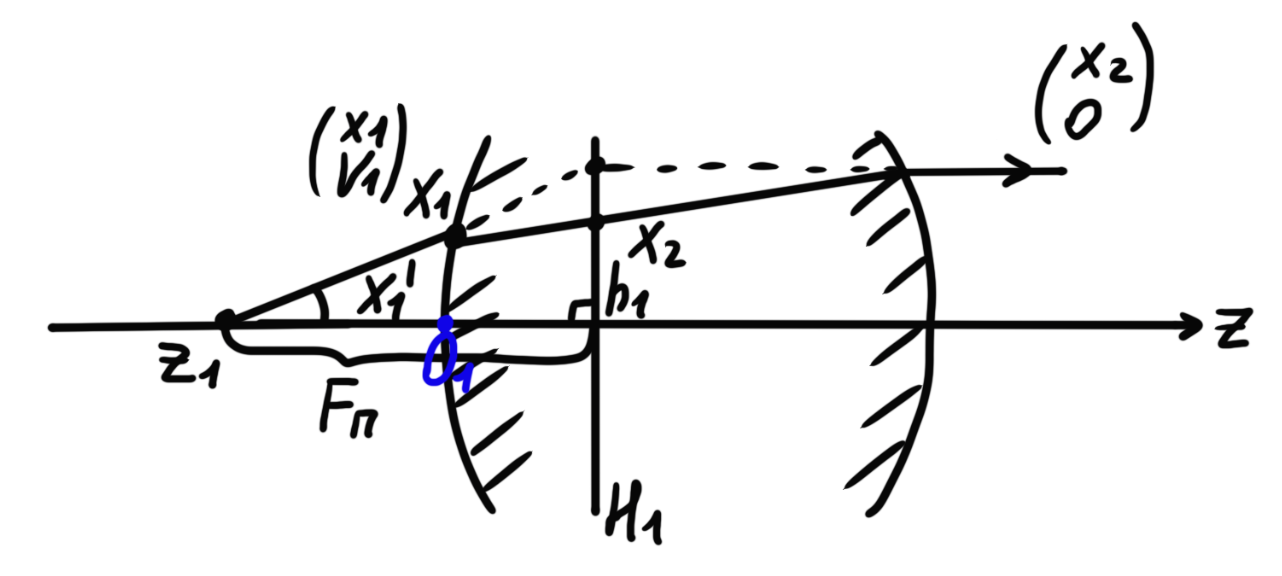
\includegraphics[width=0.55\textwidth]{/Users/vladbelousov/Desktop/Semestr_4-FP-NSU/ЭиО/Лекции_по_дням/image/83.png}
\end{center} 
\[ P_1,P_2 \text{ - узловые точки}  \] 

\textbf{Матричный формализм для немеридиальнных лучей  } 

\begin{center}
    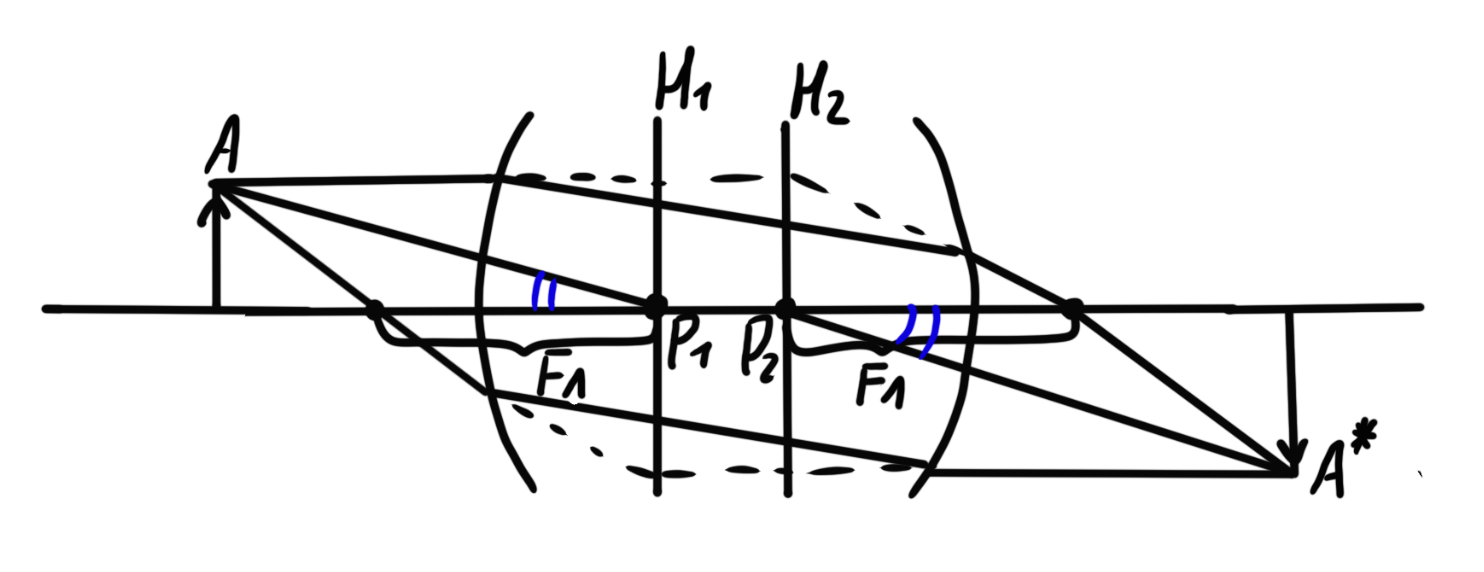
\includegraphics[width=0.6\textwidth]{/Users/vladbelousov/Desktop/Semestr_4-FP-NSU/ЭиО/Лекции_по_дням/image/84.png}
\end{center}  

Точка \( P (x,y,z) \), нормаль в точке \( P \text{ } \vec{n }  = \displaystyle (x,y,z )\frac{1}{|R|}  \). В параксиальном приближении \( \displaystyle  |x| |y| \ll |R| \Rightarrow \vec{n }  = (\frac{x}{R } , \frac{y}{R } , - 1 )\).

Граничное условие на границе раздела \( \vec{k } _{1_{\perp}  } = \vec{k}_{1_{\perp} }    \) 

\begin{center}
    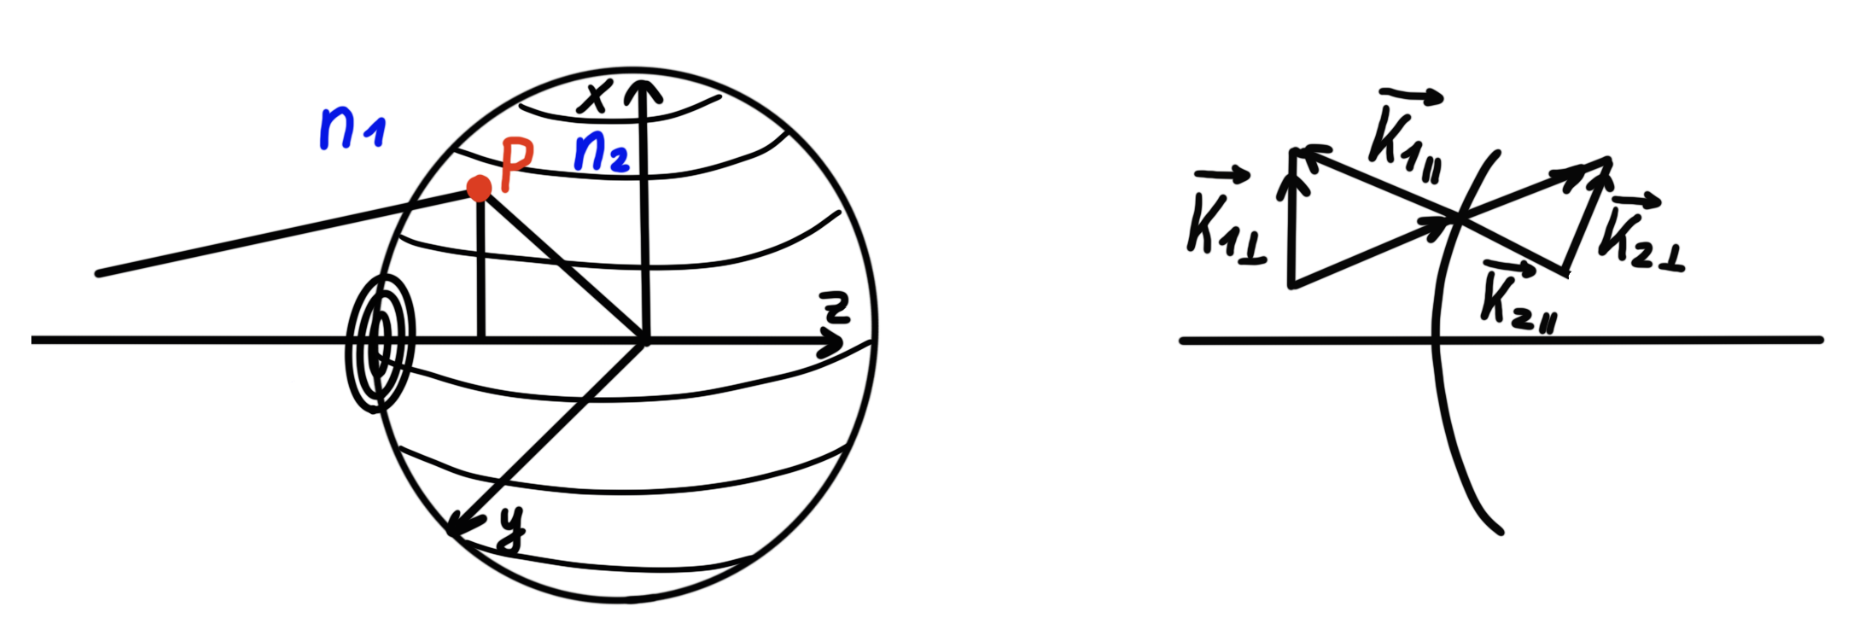
\includegraphics[width=0.6\textwidth]{/Users/vladbelousov/Desktop/Semestr_4-FP-NSU/ЭиО/Лекции_по_дням/image/85.png}
\end{center}  

\[ \vec{k }  _1 = k_0 n_1 \left( \frac{dx }{ds } , \frac{dy}{ds }  , \frac{dz}{ds}   \right)  , \quad k_0 = \frac{\omega}{c } \] 
\[ d \vec{r }  = (dx , dy ,dz ) , \text{ }  |d \vec{r }  | = ds. \text{ Если луч параксиальный, то } dz = ds  \]  
\[\Rightarrow \vec{k}_1 \approx k_0 n_1 \displaystyle \left( \frac{dx}{dz }  , \frac{dy}{dz } , 1     \right) = k_0 n_1 (x_1 ' , y_1 ', 1 ) , \text{ }  \vec{k }  _2 = k_0 n_2 (x_2' ,y_2' , 1)   \]  
\begin{center}
    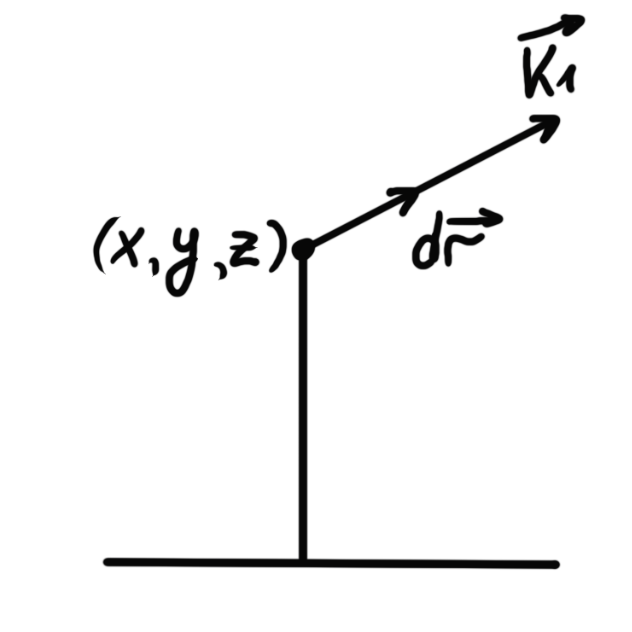
\includegraphics[width=0.25\textwidth]{/Users/vladbelousov/Desktop/Semestr_4-FP-NSU/ЭиО/Лекции_по_дням/image/86.png}
\end{center}  
\[ \vec{a} _{||} = (\vec{a } , \vec{n } )\vec{n } ,\quad  \vec{a } _{\perp } = \vec{a }  - \vec{n } (\vec{n } , \vec{a }  ) = [\vec{n } \times  [\vec{ a } \times  \vec{n} ]]   \] 
\[ \vec{k }  _{1_{\perp } } = \vec{k }  _{2_{\perp } } \Rightarrow \vec{k}_{1_{\perp } } = k_0 n_1 \bigg[ (x_1 ' , y_1 ' , 1 ) - \left( \frac{x}{R } , \frac{y}{R } , 1  \right) \bigg(\underbrace{ x_1 ' \frac{x}{R }  + y_1 ' \frac{y}{R} }_{\text{2-го порядка малости}}- 1  \bigg)\bigg]   \] 
В нашем определении \( x = x_1 = x_2 , \text{ }  y = y_1 = y_2 ; \) 
\[ \vec{k }  _{1_{\perp } } = k_0 n_1 \left( x_1 ' + \frac{x_1}{R }  , y_1 ' + \frac{y_1}{R },0  \right)  \] 

\[\vec{k}_{2_{\perp } } = k_0 n_2 \bigg[ (x_2 ' , y_2 ' , 1 ) - \left( \frac{x}{R } , \frac{y}{R } , 1  \right) \bigg(\underbrace{ x_2 ' \frac{x}{R }  + y_2 ' \frac{y}{R} }_{\text{2-го порядка малости}}- 1  \bigg)\bigg]   \] 
\[ \vec{k }  _{2_{\perp } } = k_0 n_2 \left( x_2 ' + \frac{x_1}{R }  , y_2 ' + \frac{y_1}{R },0  \right)  \] 

\[ \Rightarrow \begin{aligned}
    n_1 \left( x_1' + \frac{x_1}{R }  \right) = n_2 \left(  x_2 ' + \frac{x_2}{R}  \right) \\
    n_1 \left( y_1' + \frac{y_1}{R }  \right) = n_2 \left(  y_2 ' + \frac{y_2}{R}  \right)
\end{aligned}\] 

Для меридианного луча: 

\begin{center}
    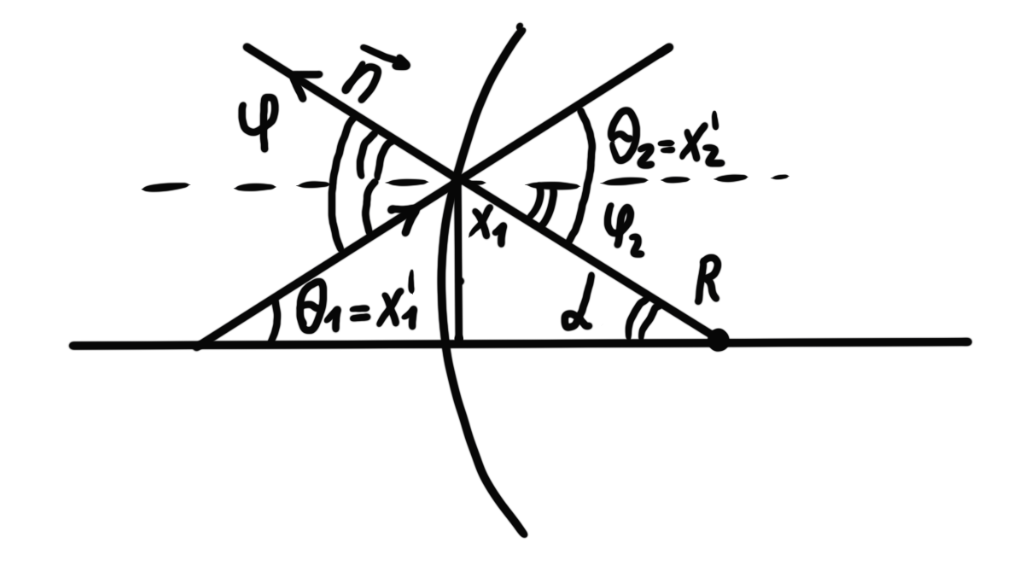
\includegraphics[width=0.6\textwidth]{/Users/vladbelousov/Desktop/Semestr_4-FP-NSU/ЭиО/Лекции_по_дням/image/87.png}
\end{center}  
Закон Снеллиуса: 

\[ n_1 \sin \left(  x_1 ' + \frac{x_1}{R }   \right) = n_2 \sin \left( x_2 '+ \frac{x_2}{R}  \right) \] 
\[ \Downarrow {\scriptstyle \left( \alpha = \mathrm{arcsin } \frac{x_1}{R} \approx \frac{x_1}{R}   \right)} \]
\[ n_1\left( x_1' + \frac{x_1}{R}  \right)= n_2 \left( x_2' + \frac{x_2}{R}  \right)\]  

\[ \begin{pmatrix}
x_2\\
x_2 '\\
y_2\\
y_2'
\end{pmatrix}  = \left( \begin{array}{l|l} \\
    M & \text{ } 0 \\ [0.2 cm]
    \hline \\
    \text{ }0 & M \\ [0.2 cm]
\end{array} \right)
\begin{pmatrix}
    x_1\\
    x_1 '\\
    y_1\\
    y_1'
\end{pmatrix}\]


\section{Теорема Лагранжа-Гельмгольца}

\begin{center}
    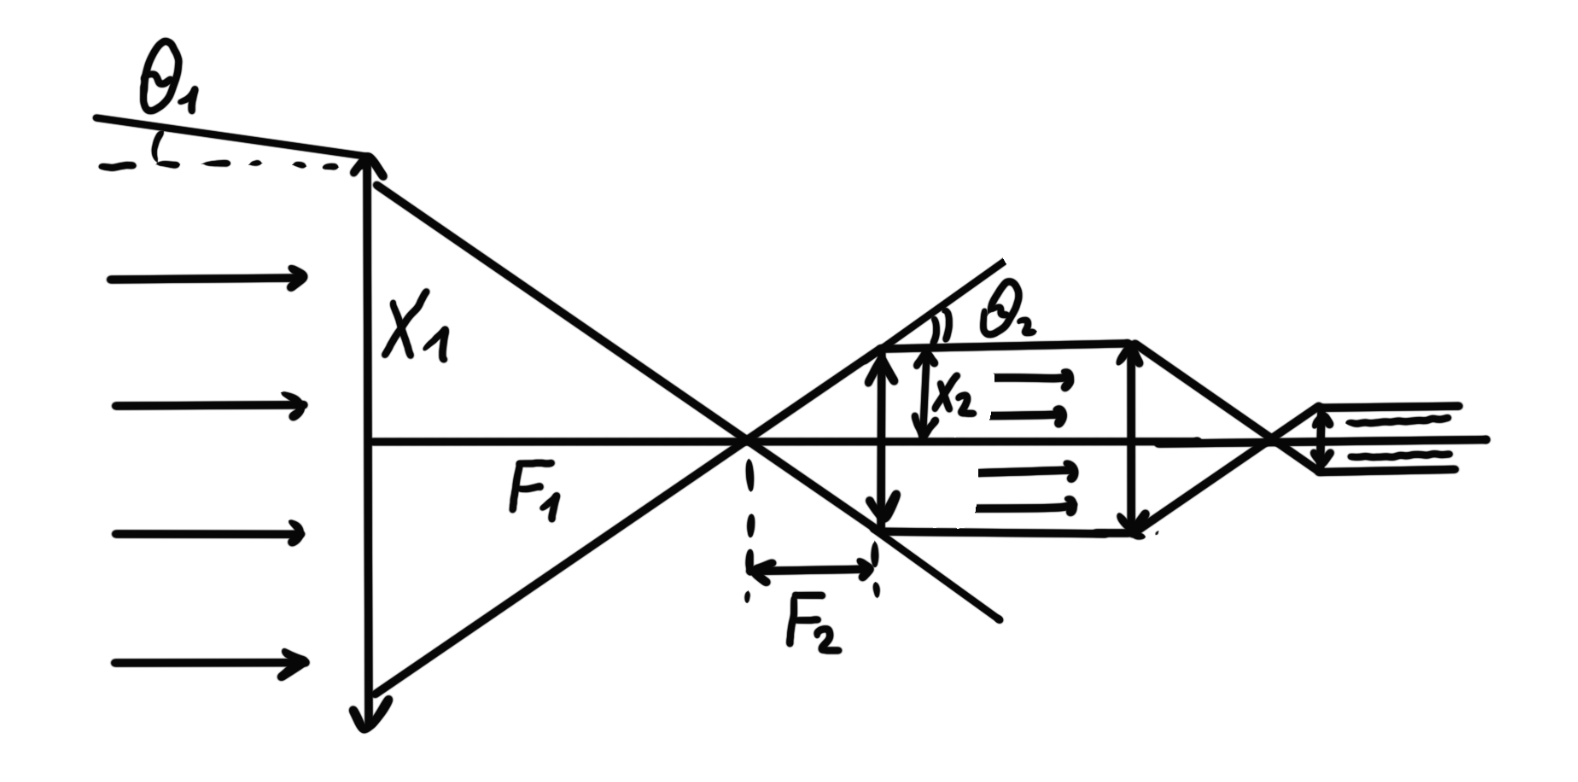
\includegraphics[width=0.6\textwidth]{/Users/vladbelousov/Desktop/Semestr_4-FP-NSU/ЭиО/Лекции_по_дням/image/88.png}
\end{center}  
Самим доказать из матричного формализма: \( n_1 x_1 \theta_1 = n_2 x_2 \theta_2  \) 

Понятие фазового портрета: 

\begin{center}
    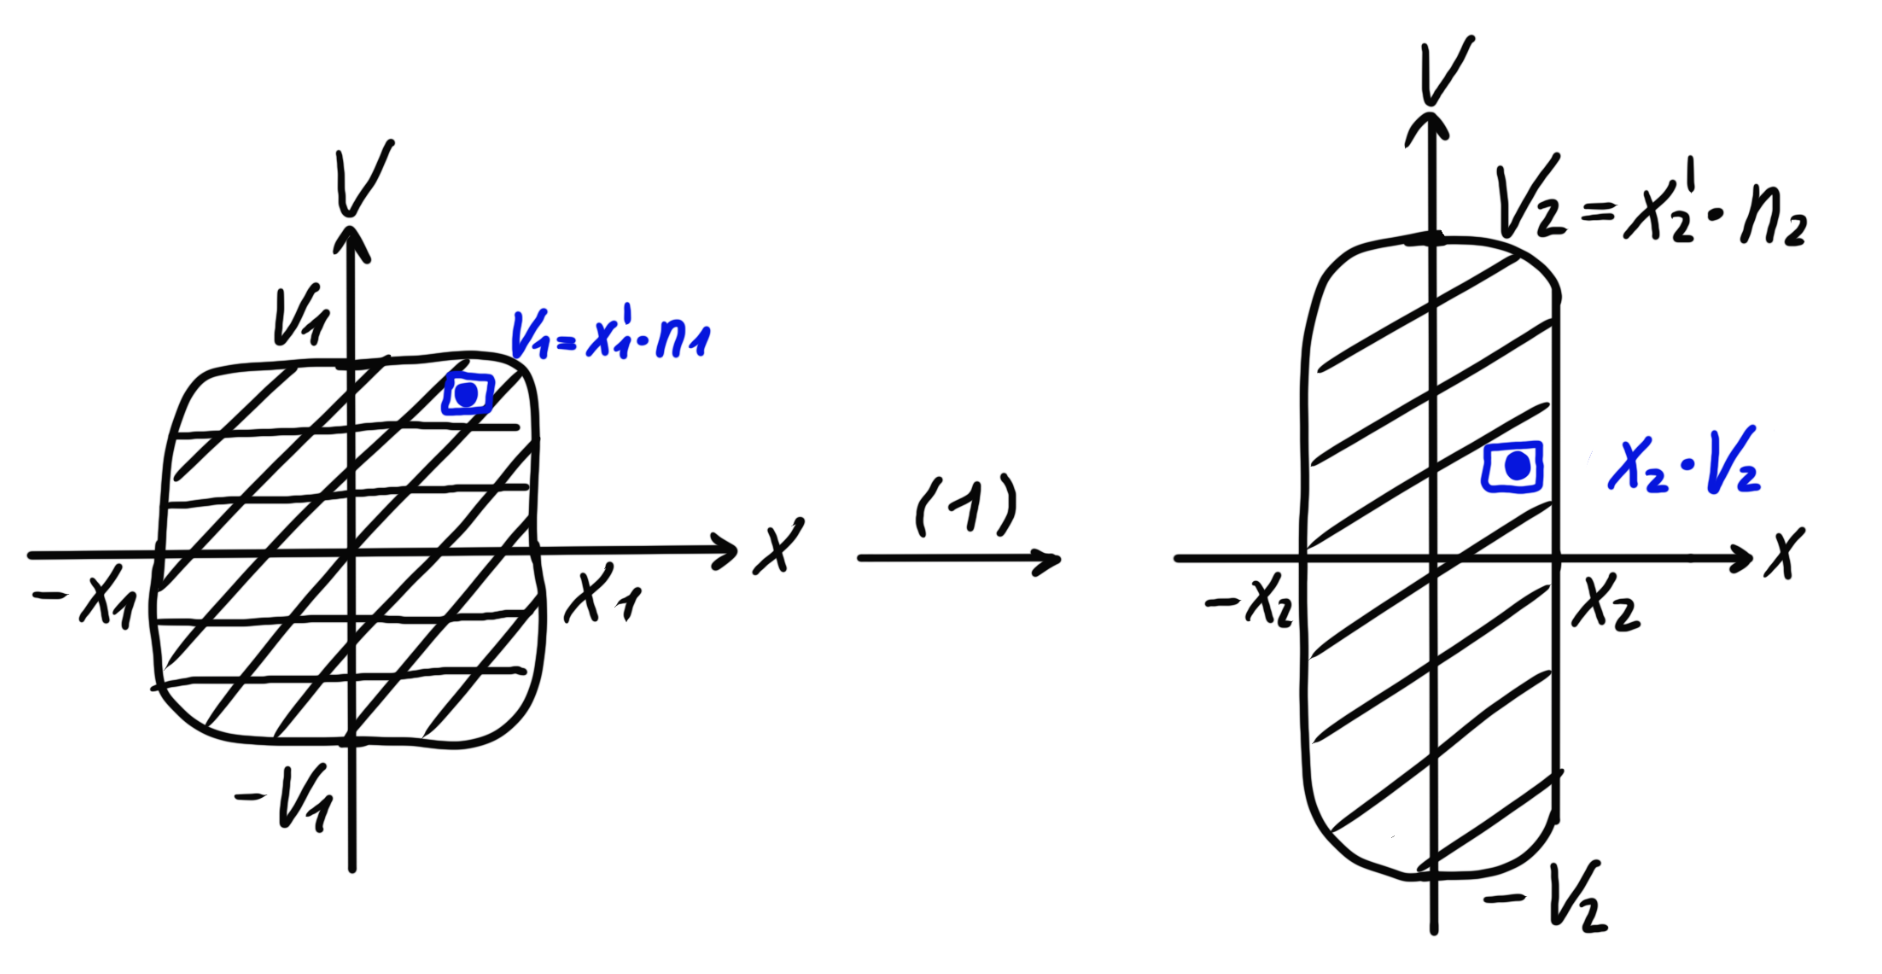
\includegraphics[width=0.7\textwidth]{/Users/vladbelousov/Desktop/Semestr_4-FP-NSU/ЭиО/Лекции_по_дням/image/89.png}
\end{center}  
\[ (1):\text{Линзы, свободное пространство, зеркала}  \] 

\begin{theorem}
    \[ \iint d x_1 d V_1 = \iint d x_2 d V_2  \] 
    \[\begin{pmatrix}
    x_2\\
    V_2
    \end{pmatrix} = \begin{pmatrix}
    &\\
    &
    \end{pmatrix} 
    \begin{pmatrix}
        &\\
        &
    \end{pmatrix} \cdot ... \cdot 
    \begin{pmatrix}
        &\\
        &
    \end{pmatrix}
    \begin{pmatrix}
        x_1\\
        V_1
    \end{pmatrix} =\begin{pmatrix}
    m_{11}  & m_{12}\\
    m_{21}& m_{22} 
    \end{pmatrix} 
    \begin{pmatrix}
        x_1\\
        V_1
    \end{pmatrix}    \] 
    \[ d x_2 d V_2  = \frac{\partial  (x_2 V_2 )}{\partial (x_1  V_1 )} d x_1 d V_1 = \det \underbrace{\begin{pmatrix}
        m_{11}  & m_{12}\\
        m_{21}& m_{22}
    \end{pmatrix} }_{= 1} d x_1 d V_1 \] 
\end{theorem} 

Минимальная угловая расходимость (у современных "хороших") лазеров: 

\[ \Delta \theta \sim \frac{\Delta k_x}{k } \sim  \frac{\pi}{k \Delta x } \sim  \frac{ \lambda }{2 \Delta x } \sim \frac{\lambda }{\Delta x } = \frac{\lambda }{2 x_1 }      \] 
, где \( \Delta k_x \)  разброс поля.

\chapter{Интерференция волн}

В оптическом диапазоне \( (f \sim  10 ^{15 }  - 10 ^{16 } \text{ Гц} ) \) большинство приборов, с которыми регистрируют электромагнитное излучение, измеряют \( <\vec{E } ^2 (t)> = I \) - интенсивность света\dots

\[ I(t ) = \frac{1}{\tau_0 } \int_{t - \frac{\tau_0}{2 } }^{t + \frac{\tau_0 }{2 } } E ^2 (t ) d t '    \] 

Если \( I  \)  не зависит от \( t  \), то \(\displaystyle  I = \frac{1}{\tau_0 } \int_{0 }^{\tau_0 } E ^2 (t ) dt '    \)  
, где \( \tau_0  \) - временное разрешение прибора (у глаза \( \tau_0   \sim 0,01 \text{ сек} \))

\textbf{Интерференция двух монохроматических волн}: 

\[ \vec{E }_1 (\vec{r },t    ) = \vec{E }  _1 (\vec{r } ) e^{ - i \omega t } , \text{ } \vec{E } _2 (\vec{r }  ,t ) = \vec{E }  _2 (\vec{r }  ) e ^{ - i \omega t }   \] 

\[ \vec{E } _{\Sigma } (\vec{r } ,t ) = (\vec{E }  _1 (\vec{r } ) + \vec{E }  _2 (\vec{r } )) e^{ - i \omega t } ,  \] 
\[ \kern-1 cm I = <(\mathrm{Re }  \vec{E } _{\Sigma } , \mathrm{Re } \vec{E } _{\Sigma}    )>  = \bigg<\left( \frac{(\vec{E } _1 + \vec{E }  _2 )e^{ -i \omega t } + (\vec{E } _1 ^ * + \vec{E }  _2 ^ * ) e^{ + i \omega t }  }{2} ,\frac{(\vec{E } _1 + \vec{E }  _2 )e^{ -i \omega t } + (\vec{E } _1 ^ * + \vec{E }  _2 ^ * ) e^{ + i \omega t }  }{2} \right) \bigg> =\] 
\[ = \frac{1}{4 }  \bigg < \bigg ( [(\vec{E } _1 + \vec{E }  _2  ) , (\vec{E } _1 ^ * + \vec{E } _2 ^ *)] + [(\vec{E } _1 + \vec{E }  _2  ), (\vec{E } _1 ^ * + \vec{E } _2 ^ *)] \bigg) \bigg > =\]  
\[= \frac{1}{2 }  \left[  |  \vec{E } _1       | ^2 + |  \vec{E } _2  | ^2 ) + 2 \mathrm{Re }  (\vec{E } _1 , \vec{E }  _2 ) \right] = I_1 + I_2 + I_{12} \] 
%%-------------------------------%%

% Закрытие документа, если файл компилируется отдельно
\ifdefined\mainfile
    % Если это основной файл, не нужно заканчивать документ
\else
    \end{document}
\fi

